\documentclass[a1]{sciposter}
\usepackage[latin1]{inputenc}
\usepackage{amsmath}
\usepackage{amssymb}
\usepackage{marvosym}
\usepackage{multicol}
\usepackage{smposter}
%\usepackage{fourier}
\usepackage{tabu}  %tablas complejas
\usepackage{blindtext}  %texto simulado, para el ejemplo solo

\newcommand\R{\mathbb{R}}
\newcommand\C{\mathbb{C}}
\newcommand{\Rp}[1]{\mathrm{Re}\,#1}
\newcommand{\Ip}[1]{\mathrm{Im}\,#1}
\newcommand\mc[1]{\mathcal{#1}}

\renewcommand{\titlesize}{\huge}
\renewcommand{\authorsize}{\Large}
\renewcommand{\instsize}{\large}

%logo de la Sección de Matemáticas en el pie, a la derecha
\renewcommand{\footlogo}{%

\includegraphics[scale=1.2]{../logo/SM.pdf}%
}



\author{Nombre Apellidos del Autor del TFG}
\title{T\'{\i}tulo del Trabajo Fin de Grado que puede llegar a ser algo bastante largo}

\institute{Facultad de Ciencias \textbullet\, Secci\'on de Matem\'aticas\\
           Universidad de La Laguna\\}
\email{alu0100xxxxxxx@ull.edu.es}

\CONV{junio}{2024}

%\renewcommand{\baselinestretch}{1.25}





\begin{document}\large
\vspace{0.15\textheight}
\maketitle


\begin{multicols}{2}


%%% Abstract
\begin{abstract}

\PARstart{P}{ }osters are widely used in the academic community, and most conferences include poster presentations in their program.  Research posters summarize information or research concisely and attractively to help publicize it and generate discussion. 

The poster is usually a mixture of a brief text mixed with tables, graphs, pictures, and other presentation formats. At a conference, the researcher stands by the poster display while other participants can come and view the presentation and interact with the author.
\end{abstract}


%%% Introduction
\section{Introduction}\label{intro}

\PARstart{E}{namorados del an\'alisis } y sin embargo ca\'oticos. No hay
nada que nos guste m\'as que una gr\'afica.

\begin{figure}
   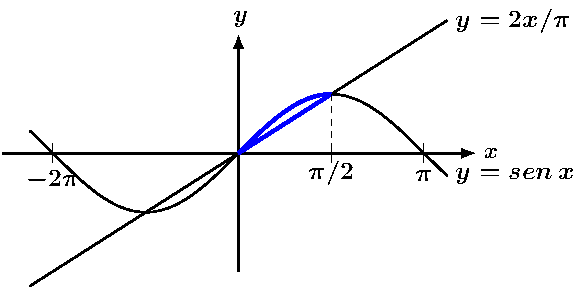
\includegraphics[scale=2.2]{../ilustraciones/fig1.pdf}
   \caption{Una gr\'afica siempre viene bien en el p\'oster.}
\end{figure}

What makes a good poster?
\begin{itemize}
 \item Important information should be readable from about 10 feet away
 \item Title is short and draws interest
 \item Word count of about 300 to 800 words
 \item Text is clear and to the point
 \item Use of bullets, numbering, and headlines make it easy to read
 \item Effective use of graphics, color and fonts
 \item Consistent and clean layout
 \item Includes acknowledgments, your name and institutional affiliation
\end{itemize}



\begin{center}
   \begin{tabular}{ r @{\hspace{1.3em}} r @{\hspace{1em}} r r }
       \textbf{A\;} & \textbf{B\;} & \textbf{C\;} & \textbf{Resto} \\
       \hline\noalign{\smallskip} 
       44.2 & 5.1 & 6.1 & 2.3\\
       712.2 & 8.3 & 99.2 & 3.1\\
       \hline
   \end{tabular}
\end{center}


%%%%%%%%%%%%%%%%%%%%%%%%%%%%%%%%%%%%%%%%%
\section{Outline}

\PARstart{W}{here do I begin?} Before try to answer these three questions:
\begin{enumerate}
 \item What is the most important/interesting/astounding finding from my research project?
 \item How can I visually share my research with conference attendees? Should I use charts, graphs, photos, images?
 \item What kind of information can I convey during my talk that will complement my poster?
\end{enumerate}

\begin{figure}[h]
  \fbox{
  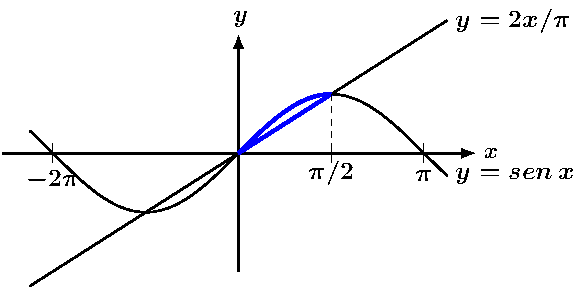
\includegraphics[scale=1.3]{../ilustraciones/fig1.pdf}\hspace{8mm}
  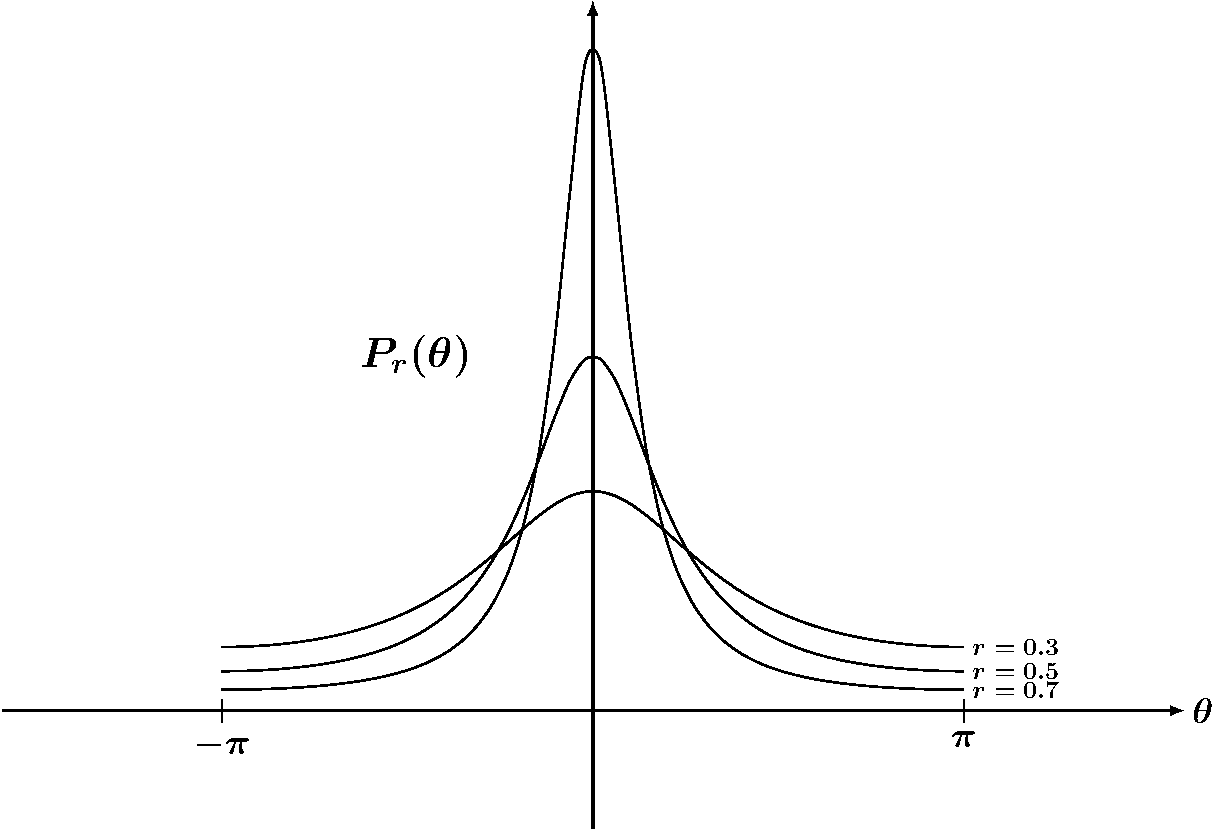
\includegraphics[scale=0.5]{../ilustraciones/fig2.pdf}\hspace{5mm}}
  \caption{Incluso m\'as de una, para comparar.}
\end{figure}
Some formulas are wellcome, but with moderation
\begin{equation*}
  \begin{split}
\text{minimize} \displaystyle\sum\limits_{j=1}^{m} w_{j}\cdot&x_{j} \\
\text{subject to} \displaystyle\sum\limits_{j:e_{i} \in S_{j}} &x_{j} \geq 1, \qquad\; i=1,\dots, n\\
                                         &x_{j} \in \{0,1\}, \;j=1,\dots, m
\end{split}
\end{equation*}


%%%%%%%%%%%%%%%%%%%%%%%%%%%%%%%%%%%%%%%%%
\section{Sections And Organization}
\PARstart{I}{t's easiest to break down} all the information you want into distinct sections, such as Background, Objectives, Methodology, Results, and Recommendations. A typical poster will have 4-8 of these sections laid out in 3 or 4 columns, but the specifics of your research will dictate which sections are important to include. Posters are read from left-to-right and top-to-bottom, so make sure to lay out your sections so they can be read in order.

\begin{center}
   \caption{\bfseries Una tabla ilustrativa de lo que se avecina}
   \tabulinesep=.2em
   \begin{tabu}{X[1.6]X[r,m]X[r,m]X[5,m] }
      \hline
      \rowfont{\bfseries} Day & Min Temp & Max Temp & \multicolumn{1}{c}{Summary} \\
      \hline
      Monday & 11\textdegree C & 22\textdegree C & 
      A clear day with lots of sunshine.  
      However, the strong breeze will bring down the temperatures.\\
      \hline
      Tuesday & 9\textdegree C & 19\textdegree C &
      Cloudy with rain, across many northern regions. Clear spells 
      across most of Scotland and Northern Ireland.\\
      \hline
      Wednesday & 10\textdegree C & 21\textdegree C & 
      Rain will still linger for the morning. Conditions will improve by early
      afternoon and continue throughout the evening. \\
      \hline
    \end{tabu}
    
    \medskip
    \caption{Una tabla a veces muestra mejor las cosas}
\end{center}


\begin{thebibliography}{1}

\bibitem{latexbook} LAMPORT, Leslie. 
\emph{\LaTeX: A Document Preparation System, User's Guide and Reference Manual.} 2nd edition.
Reading: Addison-Wesley, 1994. 

\bibitem{latexwiki}  
\emph{\LaTeX} [en l\'{\i}nea].
WikiBooks. [Consulta: 17-10-2019] Disponible en: \texttt{https://en.wikibooks.org/wiki/LaTeX}.

\bibitem{wagner}
WAGNER, C.H. Simpson's Paradox in Real Life.
\emph{The American Statistician}, 1982, vol. 36, pp. 46--48.

\end{thebibliography}

\end{multicols}
\end{document} 
